\documentclass[a4paper,12pt]{article} %style de document
\usepackage[utf8]{inputenc} %encodage des caractères
\usepackage[french]{babel} %paquet de langue français
\usepackage[T1]{fontenc} %encodage de la police
\usepackage[top=2cm,bottom=2cm,left=2cm,right=2cm]{geometry} %marges
\usepackage{graphicx} %affichage des images
\usepackage{amssymb}
\usepackage{url}
\usepackage{verbatim}
\usepackage{amsmath}

\begin{document} %début du document



%----------------------------------
%page de garde
%----------------------------------

\begin{titlepage}


\includegraphics[scale=0.3]{images/unicaen.png}

\vspace{7cm}

\begin{center}

\begin{Huge}
TPA\\
Rapport de Projet\\
\end{Huge}
\vspace{2cm}
\begin{large}
Beauchamp Aymeric 21301016\\
Chagneux Dimitri 21606807\\
Mori Baptiste 21602052\\
Leblond Valentin 21609038\\
\vspace{1cm}
L2-Info-groupe-4A
\end{large}

\end{center}
\end{titlepage}


%------------------------------
%sommaire
%------------------------------

\newpage

\tableofcontents

\newpage

%------------------------------
%contenu
%------------------------------


\section*{Objectifs}
\addcontentsline{toc}{section}{Objectifs}

\subsection*{Description du Sokoban}
\addcontentsline{toc}{subsection}{Description du Sokoban}

Le Sokoban est un jeu de réflexion de type puzzle où le joueur doit placer des caisses sur des objectifs placés à l'avance sur la carte. Le joueur gagne si toutes les caisses sont placées sur les objectifs et il ne peut pousser qu'une seule caisse à la fois. Il existe de nombreux niveaux dont la difficulté est variante.

\begin{center}
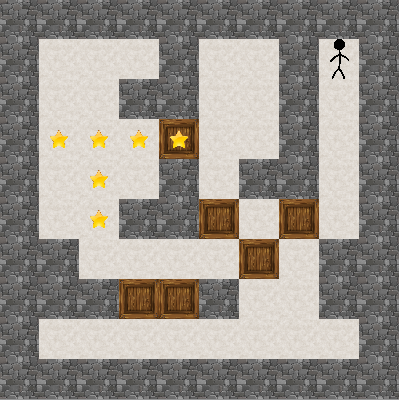
\includegraphics[scale=0.5]{images/sokoban.png}
\end{center}

\subsection*{Les fonctionnalités attendues}
\addcontentsline{toc}{subsection}{Les fonctionnalités attendues}

Pour ce projet, nous devions mettre au point une version jouable pour un humain en console, en prenant en compte l'importation de niveaux (au format \textbf{.xsb}). Il était également demandé de réaliser une interface graphique et une fonctionnalité permettant une résolution automatique de niveau.\\
Enfin, permettre de faire jouer en parallèle un humain et un ordinateur, et rendre \textit{anytime} l'algorithme de l'intelligence artificielle. C'est à dire le fait que lorsque le joueur fait un mouvement, l'intelligence artificielle doit en faire un.


\section{Fonctionnalités implémentées}

\subsection{Description des fonctionnalités}

\subsubsection*{Attendues}
\addcontentsline{toc}{subsubsection}{Attendues}

La version console fonctionne à l'aide de saisies de l'utilisateur qui lui permettent de contrôler le jeu. Une fois un niveau terminé, on demande au joueur si il souhaite passer au niveau suivant.\\

La carte est chargée à partir d'un fichier \textbf{.xsb} contenant des lignes de caractères, que l'on transforment en liste de caractères.\\
La carte est donc modélisée par des chaînes de caractères:
\begin{itemize}
\item \textbf{\#} pour un mur
\item \textbf{\$} pour une caisse
\item \textbf{@} pour le joueur
\item \textbf{.} pour un objectif
\item \textbf{*} pour une caisse sur un objectif
\item \textbf{+} pour le joueur sur un objectif
\item \textbf{espace} pour les cases vides
\end{itemize}

\begin{center}
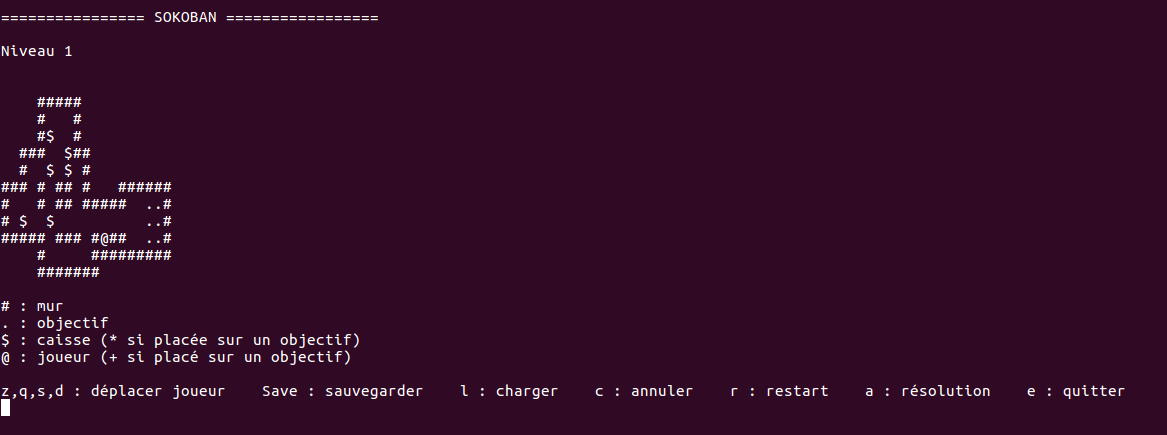
\includegraphics[scale=0.6]{images/Capture.png}\\
\end{center}

Au niveau de l'interface graphique, nous avons une zone de jeu dans laquelle on dessine le niveau et des boutons pour gérer les différentes fonctionnalités. Le personnage est déplaçable avec les flèches directionnelles ou ZQSD, si le joueur a bloqué une caisse ou si il a gagné, il ne peut plus bouger et doit recommencer le niveau ou passer au suivant (seulement si il a gagné). Si le joueur gagne, le personnage effectue le Dab et si il perd, le personnage pleure.

\begin{center}
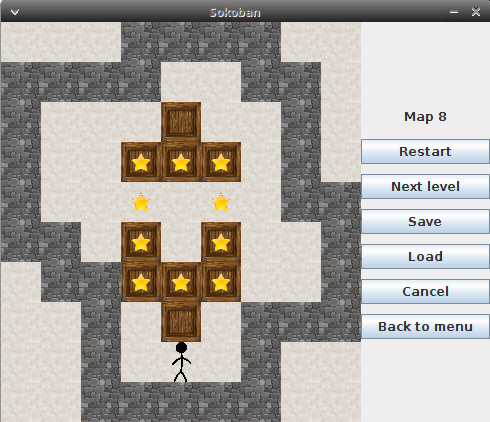
\includegraphics[scale=0.5]{images/Capture2.png}
\end{center} 

\subsubsection*{Ajoutées}
\addcontentsline{toc}{subsubsection}{Ajoutées}

Au lancement du programme, l'utilisateur peut choisir un profil ou en créer un nouveau.\\
En fonction de l'avancement du profil donné, le joueur a débloqué un certain nombre de carte, pour débloquer la carte suivante il faut finir le niveau en cours. Lorsqu'un profil est chargé, la dernière carte non terminée est lancée automatiquement.\\

Nous proposons également à l'utilisateur de sauvegarder sa partie à un instant du niveau donné, de charger sa sauvegarde (il n'y a pas de conflit entre la sauvegarde de chaque utilisateur), d'annuler le coup précédemment joué (cette fonctionnalité n'annule qu'un seul coup en arrière) et enfin de recommencer le niveau courant.

\end{document}
